\documentclass[12pt,spanish]{article}
\usepackage[spanish]{babel}
\usepackage{graphicx}
\usepackage{color}
\usepackage{colortbl}
\usepackage{amsthm,thmtools}
\usepackage{dirtytalk}
\usepackage{multirow}
\usepackage{amsmath}
\usepackage{subcaption}
\usepackage{adjustbox}
\usepackage{amsmath}
\usepackage{centernot}
\usepackage{mathtools}
\usepackage{multirow}
\usepackage[hidelinks]{hyperref}
\usepackage{caption}
\usepackage{eurosym} % para el euro
\usepackage{amsthm}
\usepackage{multicol}
\usepackage{float}
\usepackage{amsfonts}
\usepackage{titling}
\usepackage{soul}
\usepackage{listings}
\usepackage{array}
\usepackage{tikz}
\usepackage{apacite}
\usepackage{etoolbox}
\usepackage{xcolor}
\usetikzlibrary{shapes.geometric, arrows, chains, calc,positioning,fit,decorations.pathreplacing}
\usepackage[framemethod=tikz]{mdframed}

\graphicspath{ {../img/}}
\selectlanguage{spanish}
\usepackage[utf8]{inputenc}
\usepackage{graphicx}
\usepackage[a4paper,left=3cm,right=2cm,top=2.5cm,bottom=2.5cm]{geometry}

\lstset{
  breaklines=true,
  postbreak=\mbox{\textcolor{red}{$\hookrightarrow$}\space},
}

\newcommand{\quotebox}[1]{\begin{center}\fcolorbox{white}{blue!10}{\begin{minipage}{0.9\linewidth}\vspace{10pt}\center\begin{minipage}{0.8\linewidth}{\space\Huge``}{#1}{\hspace{1.5em}\break\null\Huge\hfill''}\end{minipage}\smallbreak\end{minipage}}\end{center}}

\title{Computación Ubicua e Inteligencia Ambiental}
\setlength{\droptitle}{10em}
\author{Carlos Sánchez Páez}

\makeindex
\begin{document}
\definecolor{light-gray}{gray}{0.95}
\lstset{columns=fullflexible,basicstyle=\ttfamily}
\surroundwithmdframed[
  hidealllines=true,
  backgroundcolor=light-gray,
  innerleftmargin=0pt,
  innertopmargin=0pt,
  innerbottommargin=0pt]{lstlisting}


\begin{titlepage}

 \newlength{\centeroffset}
 \setlength{\centeroffset}{-0.5\oddsidemargin}
 \addtolength{\centeroffset}{0.5\evensidemargin}
 \thispagestyle{empty}

 \noindent\hspace*{\centeroffset}
 \begin{minipage}{\textwidth}

  \centering
  
\includegraphics[width=0.9\textwidth]{logo_ugr.jpg}\\[1.4cm]

  \textsc{ \Large Computación Ubicua e Inteligencia Ambiental\\[0.2cm]}
  \textsc{GRADO EN INGENIERÍA INFORMÁTICA}\\[1cm]

  {\Huge\bfseries ARWrite \\}
 \end{minipage}

 \vspace{1.5cm}
 \noindent\hspace*{\centeroffset}
 \begin{minipage}{\textwidth}
  \centering

  \textbf{Autor}\\ {Carlos Sánchez Páez}\\[2.5ex]
  
\includegraphics[width=0.4\textwidth]{etsiit_logo.png}\\[0.1cm]
  \vspace{1.5cm}
  
\includegraphics[width=0.15\textwidth]{decsai.jpg}\\[0.1cm]
  \vspace{1cm}
  \textsc{Escuela Técnica Superior de Ingenierías Informática y de Telecomunicación}\\
  \vspace{1cm}
  \textsc{Curso 2019-2020}
 \end{minipage}
\end{titlepage}
\thispagestyle{empty}
\newpage
\tableofcontents{}
\newpage

\section{Descripción de la app}

El objetivo de este proyecto es desarrollar una aplicación basada en realidad aumentada que se utilizará para reforzar la enseñanza del trazo y la caligrafía a niños/as de infantil. Ésto se conseguirá haciendo que el usuario (niño/a) intente dibujar una letra (elegida por el profesor/a) en el aire con un puntero. El sistema identificará mediante técnicas de OCR la entrada e informará si coincide con lo esperado.\\

La aplicación constará de dos ventanas, una en la que se verá la letra objetivo y otra que mostrará la captura de video y el trazo dibujado hasta el momento.\\


\section{Motivación}

\subsection{Problema a resolver}
\label{problema}

La tecnología tiene un rol clave hoy día en prácticamente todos los ámbitos de nuestra vida. En el educativo, las clases cada vez se enriquecen más gracias a recursos digitales. Esto ocurre en prácticamente todos los sectores, desde el infantil hasta las altas titulaciones. \\

En el caso de las primeras etapas escolares de los alumnos (infantil), la enseñanza apoyada por medios digitales se hace cada vez más necesaria. En \cite{Robles-Melendez} se justifica su uso en el aula ya que potencian la motivación y comprensión de la materia para el alumno. Podemos contrastar la efectividad de las mismas en publicaciones como \cite{Bonneton-Botte2020}, que propone una aplicación para aprender a escribir en una tablet.\\

En este proyecto se pretende aprovechar la serie de ventajas que trae la tecnología al aula para conseguir que el alumno/a desarrolle el aprendizaje del trazo de una forma motivadora y amena, cambiando la tradicional escritura en pizarra por escritura en realidad aumentada.

\subsection{Competencia}

En la actualidad ya existen aplicaciones de realidad aumentada orientada a la educación de preescolar. Por ejemplo, QuiverVision \cite{quiver} ofrece una aplicación en la que el usuario colorea unas plantillas con dibujos y al enfocarlas con una tablet o smartphone, el dibujo se vuelve interactivo, ofreciendo al alumno/a jugar con el personaje que ha dibujado. Math Alive \cite{MathAlive} propone juegos que consisten en colocar cartas frente a una cámara para aprender a contar y realizar operaciones básicas.\\

Existen más aplicaciones de realidad aumentada enfocadas a la educación en preescolar, pero se centran en que el alumno/a rellene fichas y las enfoque con la cámara para hacerlas interactivas o bien. Aquí se encuentra el elemento diferenciador del proyecto: el usuario realizará el trazo frente a la pantalla y la aplicación le proporcionará un \emph{feedback}.

\begin{figure}[H]
	\centering
	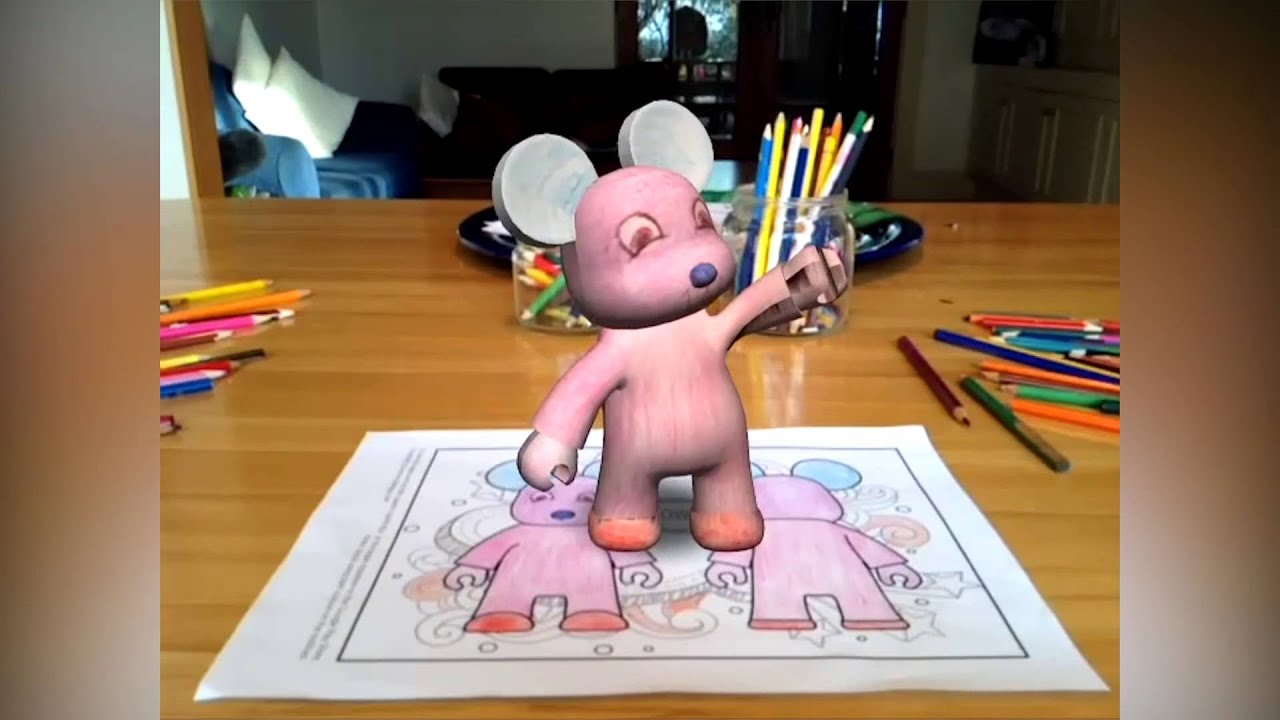
\includegraphics[scale=0.25]{quiver.jpg}
	\caption{\emph{Quiver} en funcionamiento}
\end{figure}

\subsection{Opiniones de expertos}

En la sección \ref{problema} podemos consultar varias referencias bibliográficas que avalan la efectividad de las aplicaciones de realidad aumentada en el ámbito escolar. Además, contamos con la opinión de Isabel María Páez Alba, graduada en Educación Infantil por el Centro Adscrito de Magisterio María Inmaculada de Antequera en el año 1988 y que lleva ejerciendo su profesión durante 31 años:

\quotebox{opinion goes here}

\section{Recursos a utilizar}

Para el desarrollo del proyecto se pretenden utilizar las siguientes tecnologías:
\begin{itemize}
	\item \textbf{Plataforma destino}: PC
	\item \textbf{Lenguaje de programación}: Python \cite{python}
	\item \textbf{Frameworks}
		\begin{itemize}
			\item OpenCV \cite{opencv}. Librería orientada a la visión por computador en tiempo real.
			\item Keras \cite{Keras}. Librería orientada a redes neuronales. Se utilizará junto a MNIST \cite{mnist}, una base de datos de dígitos escritos a mano para construir una red neuronal que clasificará la entrada del usuario.
		\end{itemize}
\end{itemize}

\section{Esquema}


\newpage
\bibliographystyle{apacite}
\bibliography{refs}

\end{document}
